% GFA specifications
\chapter{Le specifiche GFA}
GFA è l'acronimo per Graph Assembly Format, è un
formato per la rappresentazione dei legami presenti fra le sequenze di
un genoma al fine di riuscire a ricostruirne la struttura.
Le motivazioni che riesiedono alla base della proposta per un nuovo
formato consistono nell'uniformare le notazioni che programmi
di visualizzazione, di assemblaggio e di manipolazione potessero
utilizzare.

La prima versione della specifica GFA viene indicata col termine
GFA1. Questa prima versione mira, come vedremo successivamente,
limita la descrizione delle possibili situazioni in cui due sequenze
possono trovarsi in relazione. Per questo motivo, e per estendere
maggiormente l'insieme delle informazioni utili da descrivere,
è stata sviluppata una seconda specifica, indicata con GFA2.
Questa specifica generalizza, usando un'unica notazione,
i collegamenti fra sequenze descritti da GFA1 e permette inoltre
di descrivere relazioni fra sequenze di ogni natura.
GFA2 è un \emph{superset} di GFA1 e come tale permette
(con un minimo numero di operazioni) di trasformare un file GFA2
nell'analogo (rappresentabile) in GFA1. Questa seconda specifica
è stata appositamente pensata per permette la descrizione di
sequenze e collegamenti imponendo un minimo numero di vincoli,
permettendo all'utilizzatore di impiegarla per la descrizione di dati
indipendentemente dai dettagli che questi forniscono.

Entrambe le specifiche adoperano la stessa formattazione delle linee.
Una linea descrive un'informazione dell'assemblaggio, sia
essa una sequenza, un collegamento, un insieme di elementi o
la versione della specifica. In ogni riga, il primo carattere indica
l'identità della linea stessa cui succedono, separati esclusivamente
da tabulazioni, gli elementi che costituiscono l'informazione
che la linea descrive e che prendono il nome di \emph{campi}.
I campi possono essere definiti o meno, nel qual caso l'assenza
dell'informazione viene indicata con un asterisco \texttt{*}.

In ogni linea di entrambe le specifiche è possibile descrivere campi
opzionali (che possono essere predefiniti da una linea o introdotti
esclusivamente dall'utente), descritti nel formato \texttt{TAG:TIPO:CONTENUTO}
dove \texttt{TAG} è una sequenza di due caratteri alfanumerici
(in maiuscolo se il campo è predefinito dalla linea, in minuscolo
altrimenti) che identifica l'informazione che esso indica.
Il \texttt{TIPO} di un campo viene anch'esso descritto da un
identificatore, ciascuno indicante il seguente contenuto:

\noindent
\begin{table}[h]
	\rowcolors{1}{white}{lightgray}
	\begin{tabularx}{\textwidth}{ | X | l | }
		\hline
		Tipo	&	Descrizione\\
		A 		&	Singolo carattere stampabile(escluso lo spazio)\\
		i 		&	Intero con segno\\
		f 		&	Decimale con precisione singola\\
		Z		&	Stringa stampabile (incluso lo spazio)\\
		J		&	Stringa JSON, escludendo caratteri di newline e di tabulazione\\
		H 		&	Array di Byte in formato esadecimale\\
		B 		&	Array di interi o di decimali\\
		\hline
	\end{tabularx}
	\caption{Tabella dei tipi che è possibile usare per specificare campi opzionali.}
	\label{tab:optfield-type}
\end{table}

Mentre verranno analizzate le linee delle due specifiche, è essenziale
avere un'idea di cosa sia una sequenza e di come questa può essere in
relazione con le altre.
Con il termine sequenza viene indicata una \emph{sequenza nucleotidica},
un susseguirsi di lettere che denotano le unità molecolari che compongono
gli acidi nucleici di RNA e DNA (\emph{nucleotide}).
Una sequenza è priva di un ordine specifico, ma è possibile attribuirgliene
uno osservando la composizione del tipo di legame che collegano
gli elementi costitutivi il nucleotide, in base all'orientamento del
legame presente tra le unità di carbonio 3' di un un'unità
e la stessa unità 5' della successiva. Grazie a tale osservazione
è possibile individuare un ordinamento che verrà definito
come 3'5'.

\begin{wrapfigure} {O} {0.65\textwidth}
        \begin{centering}
                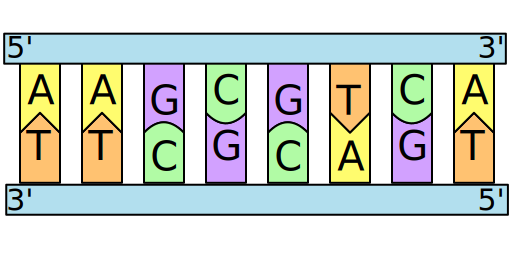
\includegraphics[scale=0.5]{dna-strand}
                \caption[Rappresentazione del DNA]{Rappresentazione grafica degli strand che compongono il DNA.}
                \label{fig:dna-strand}
        \end{centering}
\end{wrapfigure}

Oltre questa considerazione, bisogna tenere conto che
l'informazione presente nel DNA
è la stessa a parità di estremità, ma in ordine inverso e
complementato (vedi figura \ref{fig:dna-strand}) (sostituendo
la citosina con la guanina e
l'adedina con la timina). Nel caso di RNA alla timina
si sostituisce l'uracile, ma il processo di formazione del RNA
prevede anch'esso questa operazione di complementazione
della sequenza.

Ergo, quando si considera una sequenza (nel caso
dell'assemblaggio del DNA), è necessario tenere presente
che un collegamento fra due sequenze potrebbe considerare
una sequenza posta sullo strand (una delle estremità
che compone l'elica del DNA) opposto e di conseguenza una loro
sovrapposizione potrebbe richiede un preprocessamento della
stringa che la porti ad essere coerente con l'altra, operazione
che prende il nome di \emph{reverse and complement}.

% GFA1
\section{Linee GFA1}
GFA1 è la prima versione della specifica, essa si concentra nella descrizione
delle sequenze, collegate tra loro da una relazione di \emph{contenimento}
o di \emph{successione}.

Le linee previste dalla specifica sono header, segment, link, containment
e path.

L'header è una riga il cui scopo è quello di indicare la versione della specifica
in uso, può ripresentarsi più volte all'interno del file per indicare parametri
opzionali validi per tutti gli elementi. Tale linea viene indicata con il simbolo \texttt{H}.

\subsection{Segment}
La linea di Segment (indicata con il simbolo \texttt{S}) descrive in termini
generici una sequenza, la quale può essere definita o no. All'informazione
viene attribuito un identificativo che deve essere unico in tutto in file.
A queste proprietà se ne possono aggiungere altre, descritte da campi
opzionali, tra i quali si citano per ricorrenza la lunghezza (\texttt{LN}) e
il conto dei \emph{k-meri} (l'insieme di tutte le possibili sottostringhe
di lunghezza k contenute nella stringa).

\begin{lstlisting}[caption=Una possibile Segment line.]
S	5	CCCGGGGTAA		LN:i:10
\end{lstlisting}

\subsection{Link}
I Link sono il principale tipo di relazione fra due sequenze. Essi
indicano una sovrapposizione fra le sequenze indicate da due Segment.
Nello specifico, un Link fra due Segment indica che la parte terminale
della prima sequenza è coinvolta in una sovrapposizione (\emph{overlap})
con la seconda. Il termine che descrive esattamente questa situazione
è \emph{dovetail overlap}. Tale tipologia di collegamente costituisce
un'informazione di rilievo nell'analisi dell'assemblaggio poichè descrive
un ``principio'' di susseguirsi fra un insieme di sequenze.

Il link non solo descrive questa situazione, ma indica anche quale
estremità della sequenza è coinvolta nell'overlap. Ricordando che
l'informazione contenuta nella struttura elicoidale del DNA è la stessa a parità
di estremi (ma in senso inverso e complementata), è possibile
che due sequenze siano contigue (in una situazione di dovetail
overlap) considerando la loro provenienza da due estremità
diverse dell'elica (strand).
Il link permette di esprimere il collegamento considerando anche questa
particolarità; per farlo esso utilizza un segno ``\texttt{+}'' per indicare
che la sequenza non necessita di alcun processamento nel suo
coinvolgimento nella sovrapposizione, mentre utilizza un segno ``\texttt{-}''
per esplicare la necessità di effettuare un' operazione di reverse
and complement sulla sequenza prima di poterla considerare
nell'overlap.

Visto che, come dicevo poc'anzi, un Link descrive una sovrapposizione
tra la fine della prima sequenza e l'inizio della seconda (indipendentemente
dai segni associati alle due sequenze coinvolte), ciò da luogo a quattro
possibili situazioni:
\begin{itemize}
	\item la parte destra della prima sequenza si sovrappone con la parte
		sinistra della seconda (vedi figura \ref{fig:dov-ov}\subref{fig:dov-ov++});
	\item la parte destra della prima sequenza si sovrappone con la parte
		destra della seconda (vedi figura \ref{fig:dov-ov}\subref{fig:dov-ov+-});
	\item la parte sinistra della prima sequenza si sovrappone con la parte
		sinistra della seconda (vedi figura \ref{fig:dov-ov}\subref{fig:dov-ov-+});
	\item la parte sinistra della prima sequenza si sovrappone con la parte
		destra della seconda (vedi figura \ref{fig:dov-ov}\subref{fig:dov-ov--}).
\end{itemize}

\captionsetup{justification=centering}
\begin{figure}[h]
	\begin{subfigure}{.5\linewidth}
	  \centering
	  \includegraphics[scale=0.4]{dov_ov_++}
	  \caption{}
	  \label{fig:dov-ov++}
	\end{subfigure}%
	\begin{subfigure}{.5\linewidth}
	  \centering
	  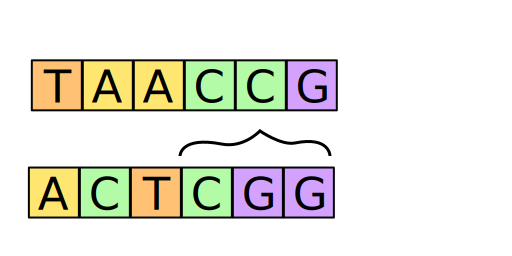
\includegraphics[scale=0.4]{dov_ov_+-}
	  \caption{}
	  \label{fig:dov-ov+-}
	\end{subfigure}%
	
	\bigskip%
	
	\begin{subfigure}{0.5\linewidth}
	  \centering
	  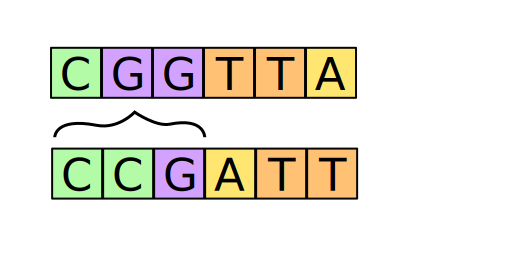
\includegraphics[scale=0.4]{dov_ov_-+}
	  \caption{}
	  \label{fig:dov-ov-+}
	\end{subfigure}%
	\begin{subfigure}{0.5\linewidth}
	  \centering
	  \includegraphics[scale=0.4]{dov_ov_--}
	  \caption{}
	  \label{fig:dov-ov--}
	\end{subfigure}
	
	\captionsetup{justification=justified}
	\caption[Rappresentazione delle posizioni situazioni di dovetail overlap]{\textit{(a)} Dovetail overlap senza bisogno di alterare le sequenze.
		\textit{(b)}  Dovetail overlap dove la seconda sequenza necessita
	  		di un'operazione di reverse and complement per sovrapporsi alla prima.
	  	\textit{(c)} Un'operazione di reverse and complement deve essere eseguita
	  		sulla prima sequenza, affinchè ci sia un overlap.
	  	\textit{(d)} Entrambe le sequenze richiedono operazioni di reverse and complement.}
	\label{fig:dov-ov}
\end{figure}

